% -*- coding: iso-latin-1 -*-
%
% SUMMARY:
% USAGE:
%
% AUTHOR:       Christophe Prud'homme
% ORG:          Christophe Prud'homme
% E-MAIL:       prudhomm@zion
%
% ORIG-DATE:  7-Apr-04 at 16:48:32
% LAST-MOD:  7-Apr-04 at 23:07:19 by Christophe Prud'homme
%
% DESCRIPTION:
% DESCRIP-END.

\date{January 21 2008}

\begin{document}

% For every picture that defines or uses external nodes, you'll have
% to apply the 'remember picture' style. To avoid some typing, we'll
% apply the style to all pictures.
\tikzstyle{every picture}+=[remember picture]
\tikzstyle{na} = [baseline=-.5ex]

%By default all math in TikZ nodes are set in inline mode. Change this to
% displaystyle so that we don't get small fractions.
\everymath{\displaystyle}

\lecture[3]{Polynomial Approximation}{approx}
\subtitle{}

\begin{frame}
  \maketitle
\end{frame}

\begin{frame}
  \tableofcontents
\end{frame}

\begin{frame}{Introduction}
  We now describe the operations on the reference element $\Omst$
  \begin{itemize}
  \item Definition of $\Omst$
  \item Construction of  polynomials
  \item Evaluation of  polynomials
  \item Differentiation of polynomials
  \item Other operation: addition, substraction, integration, $\nabla
    \cdot$, $\nabla \times$, ...
  \end{itemize}
\end{frame}

\section{Geometry}
\label{sec:geometry}


\begin{frame}[containsverbatim]{Reference Convex ${K}$}
  \begin{columns}[c]
    \begin{column}{.4\textwidth}
      \begin{figure}[H]
        \centering
        %% \movie[externalviewer=kaffeine,label=diphase]{\pgfuseimage{tetra-2}}{}
        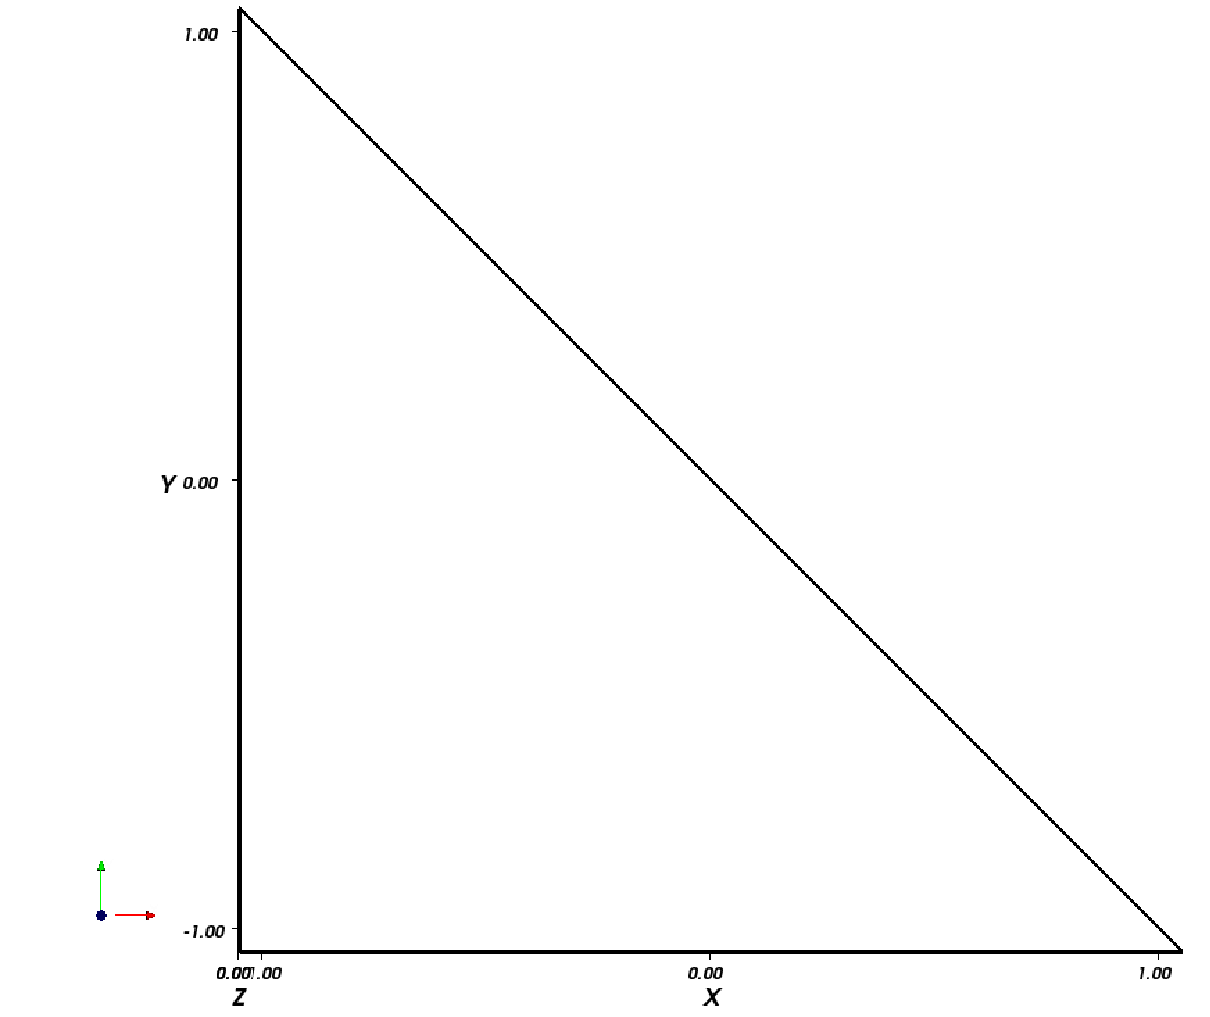
\includegraphics[width=\figwidth\textwidth]{../figures/triangle.pdf}\\
        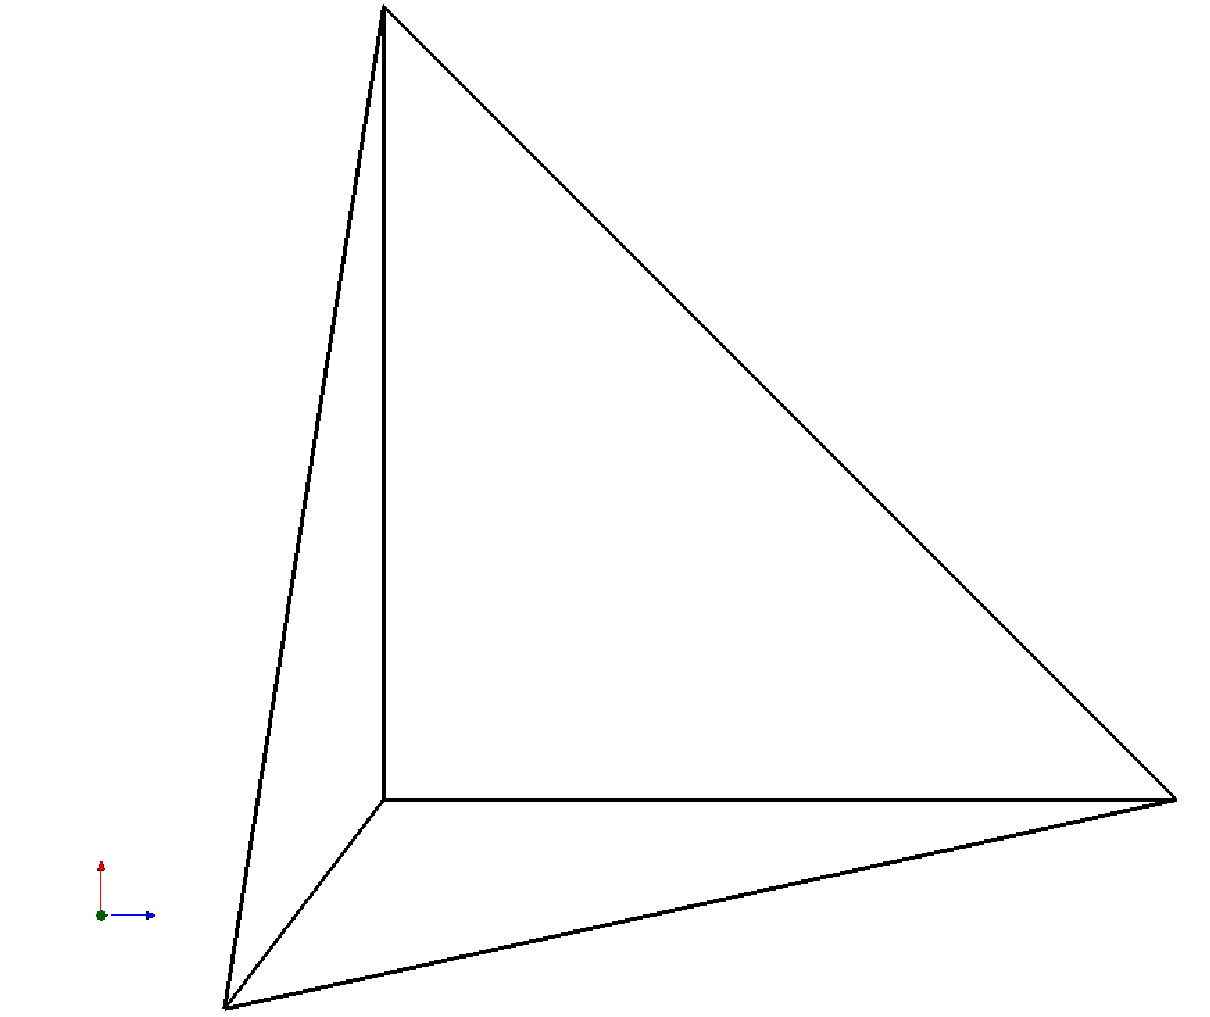
\includegraphics[width=\figwidth\textwidth]{../figures/tetra.pdf}
        %% \hyperlinkmovie[externalviewer=kaffeine]{diphase}{\beamergotobutton{Film}}
        \caption{Simplexe de R�f�rence en 2D/3D}
      \end{figure}
    \end{column}
    \begin{column}{.6\textwidth}
      \begin{block}{}
        \begin{itemize}
        \item Simplices, $d=1,2,3$
          \alert{collapsed coordinates}
        \item Simplex products
        \item Orientation
        \item Normals, Tangents
        \end{itemize}
      \end{block}
      \begin{alertblock}{Crucial}
        Decomposition of convexes into its sub-entities (volume,
        faces, edges, points) and in an ordered manner
      \end{alertblock}


% \begin{lstlisting}[]
% template<uint16_type Dim,
%          uint16_type Order = 1,
%          uint16_type RealDim = Dim,
%          typename T = double>
% class Simplex {
%  // Informations statiques
%  // orientation
%  // points
%  // points par entit�s g�om�triques
%  // normales/tangentes
%  // ...
% };
% \end{lstlisting}
    \end{column}
  \end{columns}
\end{frame}
\subsection{Interval}
\begin{frame}[containsverbatim]{The interval $[-1;1]$}
  An interval is composed of
  \begin{itemize}
  \item two vertices
  \item an edge connecting the two vertices
  \end{itemize}
  \begin{figure}[H]
    \centering
    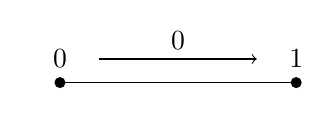
\begin{tikzpicture}[scale=2]
      \tikz {
        \fill (0,0) circle (2pt) node[above=2pt] {0};
        \draw (0,0)  to[line to] (3,0);
        \draw[->] (0.5,0.3)  to[line to] node[above] {0} (2.5,0.3) ;
        \fill (3,0) circle (2pt) node[above=2pt] {1};
      }
    \end{tikzpicture}
    \caption{Local and global numbering of the interval}
  \end{figure}
  Denote \lstinline!entity[0]! and \lstinline!entity[1]! the
  subentities sets for the vertices and edges respectively, we have
  \begin{itemize}
  \item \lstinline!entity[0] = {0,1}!
  \item \lstinline!entity[1] = {0}!
  \end{itemize}
\end{frame}

\subsection{Quadrilateral}
\begin{frame}[containsverbatim]{Quadrilateral}
  \begin{figure}[H]
    \centering
    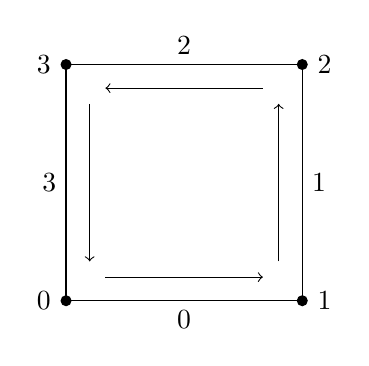
\begin{tikzpicture}[scale=1]
        \draw[->] (0.5,0.3)  to[line to]  (2.5,0.3) ;
        \draw[->] (2.7,0.5)  to[line to]  (2.7,2.5) ;
        \draw[->] (2.5,2.7)  to[line to]  (0.5,2.7) ;
        \draw[->] (0.3,2.5)  to[line to]  (0.3,0.5) ;


        \draw
        (0,0)  to[line to] node[below] {0} (3,0)
        (3,0)  to[line to] node[right] {1} (3,3)
        (3,3)  to[line to] node[above] {2} (0,3)
        (0,3)  to[line to] node[left]  {3} (0,0)
        ;
        \fill (0,0) circle (2pt) node[left=2pt] {0};
        \fill (3,0) circle (2pt) node[right=2pt] {1};
        \fill (3,3) circle (2pt) node[right=2pt] {2};
        \fill (0,3) circle (2pt) node[left=2pt] {3};
    \end{tikzpicture}

    \caption{Local numbering and orientation  for vertices and edges of the quadrilateral}
    \label{fig:2}
  \end{figure}
  We shall denote
  \begin{equation}
    \label{eq:2}
    \mathcal{Q}^2 = \{ (x_1, x_2) \in \setR{2} | -1 < x_1, x_2 < 1 \}
  \end{equation}
  We have for the quadrangle
  \begin{itemize}
  \item \lstinline!entity[0] = {0,1,2,3}!
  \item \lstinline!entity[1] = {0,1,2,3}!
  \item \lstinline!entity[2] = {0}!
  \end{itemize}
\end{frame}

\subsection{Triangle}
\begin{frame}[containsverbatim]{Triangles}
  \begin{figure}[H]
    \centering
    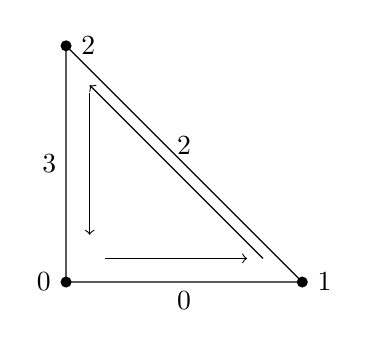
\begin{tikzpicture}[scale=1]
      \draw[->] (0.5,0.3)  to[line to]  (2.3,0.3) ;
      \draw[->] (2.5,0.3)  to[line to]  (0.3,2.5) ;
      \draw[->] (0.3,2.4)  to[line to]  (0.3,0.6) ;


      \draw
      (0,0)  to[line to] node[below] {0} (3,0)
      (3,0)  to[line to] node[above] {2} (0,3)
      (0,3)  to[line to] node[left]  {3} (0,0)
      ;
      \fill (0,0) circle (2pt) node[left=2pt] {0};
      \fill (3,0) circle (2pt) node[right=2pt] {1};
      \fill (0,3) circle (2pt) node[right=2pt] {2};
    \end{tikzpicture}

    \caption{Local numbering and orientation  for vertices and edges of the triangles}
    \label{fig:2}
  \end{figure}
  We shall denote
  \begin{equation}
    \label{eq:1}
    \mathcal{T}^2 = \{ (x_1, x_2) \in \setR{2} | -1 < x_1, x_2 < 1, x_1 + x_2 < 0 \}
  \end{equation}
  We have for the triangle
  \begin{itemize}
  \item \lstinline!entity[0] = {0,1,2}!
  \item \lstinline!entity[1] = {0,1,2}!
  \item \lstinline!entity[2] = {0}!
  \end{itemize}
\end{frame}

\subsection[Tet. and Hex.]{Tetrahedron and hexahedron}
\begin{frame}{Tetrahedron and hexahedron}
  We do a similar construction for the tetrahedron and hexahedron, i.e
  decompsoing it into vertices, edges, faces and volumes

  We shall denote
  \begin{equation}
    \label{eq:3}
    \mathcal{T}^3 = \{ (x_1, x_2, x_3) \in \setR{3} | -1 < x_1, x_2, x_3 < 1, x_1 + x_2 + x_3 < 0 \}
  \end{equation}
  and
  \begin{equation}
    \label{eq:4}
    \mathcal{Q}^3 = \{ (x_1, x_2, x_3) \in \setR{4} | -1 < x_1, x_2, x_3 < 1 \}
  \end{equation}
\end{frame}

\begin{frame}[containsverbatim]{C++}
\begin{lstlisting}
 template<uint16_type Dim,
          uint16_type RealDim = Dim>
 class Simplex {
  // static Informations
  // orientation
  // normales/tangentes
  // decomposition in subentities
  // routine to manipulate the subentities
 };
\end{lstlisting}

\end{frame}
\section{Polynomials Bases}
\label{sec:polynomials-bases}

\subsection[Space]{Polynomial Spaces}
\begin{frame}{Polynomial Spaces}
  Denote
  \begin{equation}
    \label{eq:5}
    \PS{N}(\GT{d}) = \{ p | \text{degree} \leq N \}
  \end{equation}
  and
  \begin{equation}
    \label{eq:6}
    \QS{N}(\GQ{d}) = \{ p | \text{degree} \leq N \text{ in each variable} \}
  \end{equation}
\end{frame}

\subsection[Jacobi]{Jacobi Polynomials}
\begin{frame}{Jacobi Polynomials}

  The Jacobi polynomials $P_k^{(\alpha,\beta)}$ of indices
  $\alpha,\beta > -1$ and degree $k \geq 0$ are a family of orthogonal
  polynomials on $(-1,1)$ w.r.t the inner product:
  \begin{equation}
    \label{eq:7}
    (u,v)_{(\alpha,\beta)} = \int_{-1}^1 \ u(x)\ v(x)\ (1-x)^\alpha\ (1+x)^\beta\ dx
  \end{equation}

  The polynomials can be calculated using the recurrence formulas [see Sherwin-Karnyadakis].

  \begin{block}{Remark}
    We are going to use the Jacobi polynomials using specific values
    of $\alpha$ and $\beta$. Note also that the \alert{roots} of these
    polynomials are crucial in the construction of quadrature formulas
    (we come back later to them)
  \end{block}
\end{frame}

\begin{frame}{Recurrence relations for evaluation}
  \begin{equation*}
    \label{eq:15}
  \begin{aligned}
    P_0^{\alpha,\beta}( x ) &= 1,\\
    P_1^{\alpha,\beta}( x ) &= \frac{1}{2}\Big[ \alpha -\beta +(\alpha+\beta+2)x \Big],\\
    a^1_n P_{n+1}^{\alpha,\beta}( x ) &= (a^2_n +a^3_n x) P_{n}^{\alpha,\beta}( x ) - a^4_n P_{n-1}^{\alpha,\beta}( x )\\
    a^1_n & = 2(n+1)(n+\alpha+\beta+1)(2n+\alpha + \beta)\\
    a^2_n & = (2n+\alpha+\beta+1)(\alpha^2 - \beta^2)\\
    a^3_n & = (2n+\alpha+\beta)(2n+\alpha + \beta+1)(2n+\alpha + \beta+2)\\
    a^4_n & = 2(n+\alpha)(n+\beta)(2n+\alpha + \beta+2)
  \end{aligned}

  \end{equation*}

  Some special values

  \begin{equation*}
    \begin{aligned}
      P_{n}^{\alpha,\beta}( 1 ) & =
      \begin{pmatrix}
        n+\alpha\\
        n
      \end{pmatrix} =
      \frac{(n+\alpha)!}{\alpha!n!}\\
      P_{n}^{\alpha,\beta}( -x ) & = (-1)^n P_{n}^{\alpha,\beta}( x )
    \end{aligned}

  \end{equation*}
\end{frame}
\begin{frame}{Recurrence relations for diffentiation}
  \begin{equation*}
    \label{eq:15}
  \begin{aligned}
    b^1_n \frac{d}{dx} P_n^{\alpha,\beta}( x ) &= b^2_n P_{n}^{\alpha,\beta}( x ) + b^3_n P_{n-1}^{\alpha,\beta}( x )\\
    b^1_n & = (2n+\alpha + \beta)(1-x^2)\\
    b^2_n & = n\Big[ \alpha -\beta -(\alpha+\beta+2n)x \Big]\\
    b^3_n & = 2(n+\alpha)(n+\beta)
  \end{aligned}
  \end{equation*}

\end{frame}

\begin{frame}{Gauss-Type integration}
  Integration of $u(x)$ in the interval $[-1;1]$ with respect to the function
  \begin{equation}
    \label{eq:16}
    (1-x)^\alpha (1+x)^\beta,\quad \alpha > -1,\ \beta > -1
  \end{equation}
  can be numerically evaluated using Gauss-Type integration in a discrete summation
  \begin{equation}
    \label{eq:17}
    \int_{-1}^1 (1-x)^\alpha (1+x)^\beta u(x) dx = \sum_{q=0}^{Q-1} w_q^{\alpha,\beta} u(x^{\alpha,\beta}_q) + R(u)
  \end{equation}
  where $R(u) = 0$ if $u(x) \in \mathbb{P}_{2Q-k}([-1;1])$. The value
  of $k$ is determined the type of quadrature used
  \begin{itemize}
  \item $k=1$ classical Gauss
  \item $k=2$ Gauss Radau
  \item $k=3$ Gauss Lobatto
  \end{itemize}
\end{frame}

\begin{frame}{Gauss type quadratures}
  \begin{itemize}
  \item Gauss-Jacobi (or Gauss Legendre if $\alpha=\beta=0$) does not
    restrict where the points are placed on $[-1;1]$, the
    $x^{\alpha,\beta}_q$ are the roots of $P_Q^{\alpha,\beta}([-1;1])$

  \item Gauss-Radau  places a restriction on one point
    \begin{equation}
      \label{eq:18}
      x_q =
      \begin{cases}
        -1 & q = 0\\
        x^{\alpha,\beta+1}_{q,Q-1} & q = 1,...,Q-1
      \end{cases}

    \end{equation}

      \item Gauss-Lobatto  places a restriction on two points
    \begin{equation}
      \label{eq:19}
      x_q =
      \begin{cases}
        -1 & q = 0\\
        x^{\alpha+1,\beta+1}_{q,Q-2} & q = 1,...,Q-2\\
        1 & q = Q-1\\

      \end{cases}

    \end{equation}

  \end{itemize}
\end{frame}

\begin{frame}[containsverbatim]{Computing the roots of $P^{\alpha,\beta}_N(x)$}
  To compute the $N$ roots of $P^{\alpha,\beta}_N(x)$, we use a
  Newton-Raphson algorithm with polynomial deflation and the Chebichev points ($x^{-1/2,-1/2}_{k,N}$)
  as follows:

  \begin{lstlisting}[mathescape]
    do $k=0,...N-1$
      $r = x^{-1/2,-1/2}_{k,N}$
      if ( $k$ > 0 ) $r = (r +x_{k-1})/2$
      do $j=1,...$
      $s = \sum_{i=0}^{k-1}\ 1/({r-x_i})$
      $\delta = - P^{\alpha,\beta}_N(r)/(\Big[ P^{\alpha,\beta}_N(r)\Big]' - P^{\alpha,\beta}_N(r)s)$
      $r = r + \delta$
      if ( $\delta < \epsilon$ ) exit loop
      continue
      $x_k = r$
   continue
  \end{lstlisting}
  see \lstinline!jacobi.hpp:roots()!
\end{frame}

\subsection[Moment]{Moment basis}
\label{sec:moment-basis}

\begin{frame}{Moment basis}
  The moment basis is the canonical basis for the spaces $\PS{N}(\GT{d})$ or $\QS{N}(\GQ{d})$
  \begin{equation}
    \label{eq:8}
    \PS{N}(\GT{d}) =
    \begin{cases}
      x^i, & i \leq N,\\
      x^i y^j & i+j \leq N, \\
      x^i y^j  z^k & i+j+k \leq N,
    \end{cases}
  \end{equation}
  and
  \begin{equation}
    \label{eq:9}
    \QS{N}(\GQ{d}) =
    \begin{cases}
      x^i, & i \leq N,\\
      x^i y^j & i,j \leq N, \\
      x^i y^j z^k & i,j,k \leq N,
      \end{cases}
  \end{equation}

  \begin{block}{Remarks}
    \begin{description}
    \item[GOOD] Easy to construct and compute
    \item[GOOD] Easy Integration, differentiation
    \item[GOOD] Hierarchical basis
    \item[BAD] Very bad Vandermonde matrix conditioning as polynomial degree increases
    \item[BAD] Very bad mass matrix conditioning as polynomial degree increases
    \end{description}
  \end{block}
\end{frame}

\subsection{Legendre}
\begin{frame}{Tensorized Legendre Basis}
  Take $\alpha = \beta = 0$ in the Jacobi polynomials definition. we
  denote $L_k$ the $k$-th Legendre polynomial. $(L_k)_{k=0,...,N^d}$
  form a basis of $\QS{N}(\GQ{d})$.

  \begin{figure}[H]
    \centering
    \subfigure[Legendre]{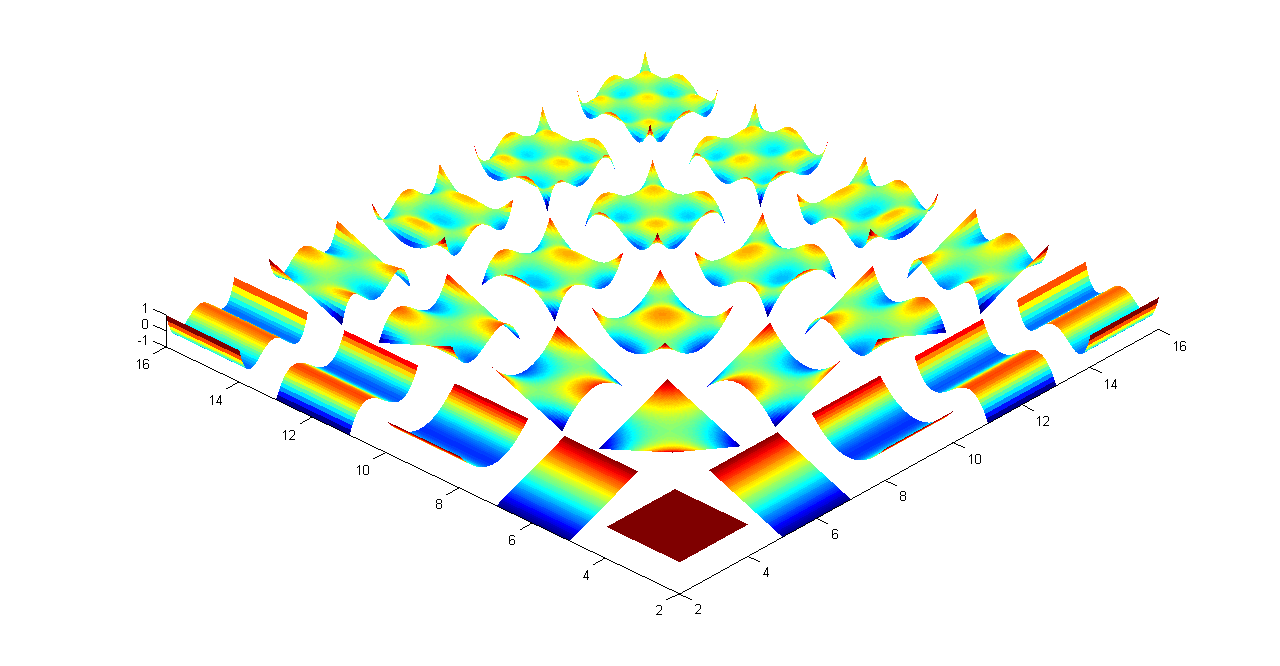
\includegraphics[width=\figwidth\textwidth]{../figures/Jacobi_2D}}
    \caption{Legendre polynomials in 2D and basis of $\QS{4}(\GQ{2})$. }
    \label{fig:3}
  \end{figure}
\end{frame}

\begin{frame}{Construction}
  \begin{itemize}
  \item The extension of 1D basis to quadrilaterals or hexahedra is done by \alert{tensorisation}.
  \item Consider $d$ 1D basis $\{ \varphi^{(l)}_{k_l}\}_{l=1}^d$ defined in $\GQ{1}$, the family $\{\phi_{\mathbf{k}}(\mathbf{x})\}_k$  given by
    \begin{equation}
      \label{eq:10}
      \phi_{\mathbf{k}}(\mathbf{x}) = \Pi_{l=1}^d\ \varphi^{(l)}_{k_l}( x_l ),\quad \mathbf{k} = (k_1,...,k_d), \mathbf{x}=(x_1,...,x_d)
    \end{equation}
    is a basis of $\QS{N}(\GQ{d})$
  \end{itemize}
  \begin{block}{Remark}
    \begin{description}
    \item[MODERATE BAD] moderate construction complexity
    \item[GOOD] $L_2$ orthogonal (normal) basis
    \item[GOOD] Hierarchical basis
    \item[GOOD] good (constant) mass matrix conditioning as polynomial degree increases
    \end{description}
  \end{block}
\end{frame}


\subsection{Dubiner}
\begin{frame}{Dubiner Basis}

  The Dubiner basis is an orthogonal modal basis on the simplices
  $\GT{d}$. Their construction derives from Legendre by collapsing
  vertices (i.e. introducing a collaped coordinate system)

  \begin{eqnarray}
    \label{eq:11}
    m: \GT{2} \mapsto \GQ{2},& (x_1,x_2) \rightarrow (\xi_1, \xi_2) &= \Big( 2\frac{1+x_1}{1-x_2}-1, x_2 \Big)\\
    m^{-1}: \GQ{2} \mapsto \GT{2},& (\xi_1,\xi_2) \rightarrow (x_1, x_2) &= \Big( \frac{1}{2}(1+\xi_1)(1-\xi_2)-1,\xi_2\Big)
  \end{eqnarray}

  We define now on the interval the following \alert{principal} functions
  \begin{equation}
    \label{eq:12}
    \left.
      \begin{array}{l}
	\psi_{p}(\xi) = P_{p}^{(0,0)}(\xi) \\
	\psi_{pq}(\xi) = \Big(\frac{1-\xi}{2}\Big)^{p}P_{q}^{(2p+1,0)}(\xi) \\
	\psi_{pqr}(\xi) = \Big(\frac{1-\xi}{2}\Big)^{p+q}P_{r}^{(2p+2q+2,0)}(\xi)
      \end{array}
    \right.
  \end{equation}
  The Dubiner basis reads in 2D and 3D as follows:
  \begin{equation}
    \label{eq:14}
    \begin{array}[c]{rl}
    \phi_{k_1,k_2}(x_1,x_2) &= \psi_{k_1}(\xi_1)	\psi_{k_1,k_2}(\xi_2)\\
    \phi_{k_1,k_2,k_3}(x_1,x_2,x_3) &= \psi_{k_1}(\xi_1)	\psi_{k_1,k_2}(\xi_2) \psi_{k_1,k_2,k_3}(\xi_3)
  \end{array}
  \end{equation}

\end{frame}
\begin{frame}{Dubiner basis in 2D}
  The cardinality is $(N+1)(N+2)/2$ in 2D and $(N+1)(N+2)(N+3)/6$ in 3D.
  \begin{figure}[H]
    \centering
    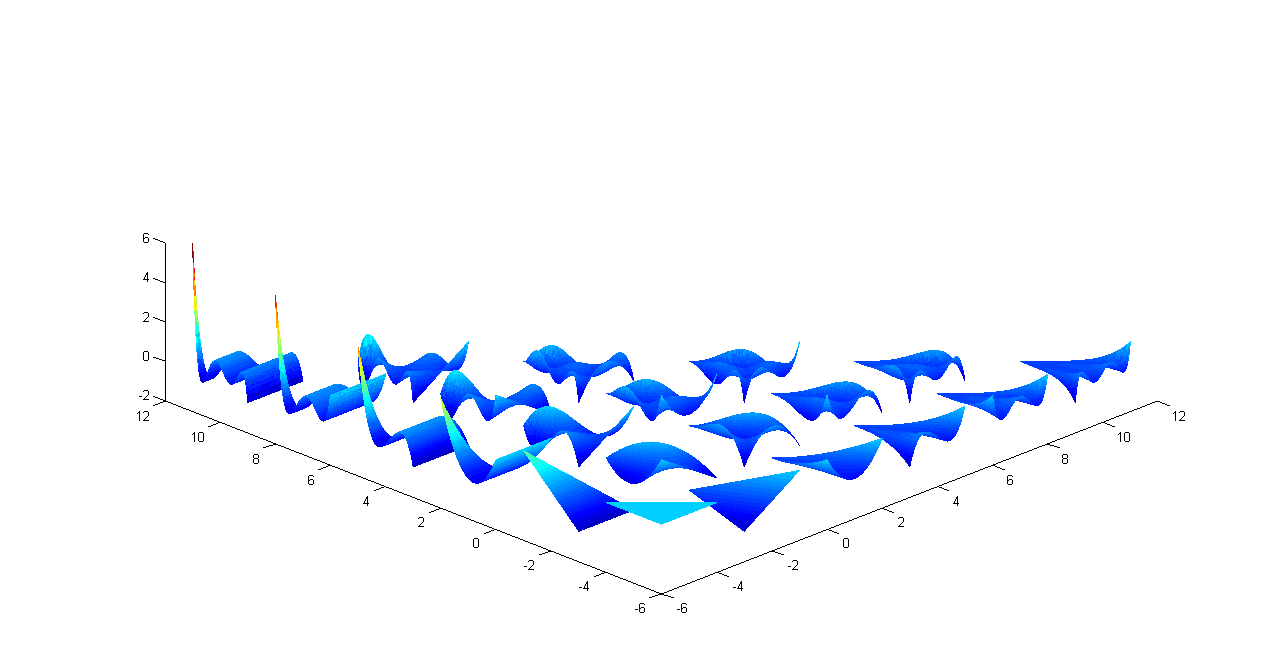
\includegraphics[width=\figwidth\textwidth]{../figures/Dubiner_5}
    \caption{Dubiner polynomials in 2D and basis of $\PS{5}(\GQ{2})$. }
    \label{fig:3}
  \end{figure}
\end{frame}

\section[FEM]{Finite element method}
\label{sec:finite-elem-meth}


\begin{frame}{Objective}

  \begin{block}{Finite/Spectral-hp element in 1/2/3D}
    \centerline{Construct {\LARGE$ (\ {K},\ {\mathbb{P}},\ {\Sigma}\ )$}}

    \begin{itemize}
    \item ${K}$ Reference convex
    \item ${\mathbb{P}}$ polynomial space
    \item ${\Sigma}$ dual space (degrees of freedom)
    \end{itemize}
    \hfill (Ciarlet, Ern \& Guermond, R.C. Kirby(Fenics/FIAT),
    Sherwin/Karniadakis, Quarteroni et al.)
  \end{block}

  % \begin{alertblock}{Standards}
  %   \begin{itemize}
  %   \item Le formalisme math�matique ci-dessus est rarement
  %     pr�sent/explicite dans les codes
  %   \item Souvent les �l�ments sont cod�s explicitement
  %     \begin{itemize}
  %     \item extension ordre �lev� difficile
  %     \item certains �l�ments rarement/jamais utilis�s car trop
  %       complexes ou pas de forme explicite
  %     \end{itemize}
  %   \end{itemize}
  % \end{alertblock}

  \note{\begin{itemize}
    \item G�om�trie �l�mentaire sur des convexes $\subset \mathbb{R}^d$
      (simplexes et produits de simplexes)
    \item Construction de familles de points dans les convexes de
      r�f�rences
    \item Construction de familles de polyn�mes sur les convexes de
      r�f�rences
    \item Construction d'un langage pour les formulations
      variationnelles
    \end{itemize}}
\end{frame}

\subsection{Point sets}

\begin{frame}{Points Sets in a Convex}

\begin{columns}
  \begin{column}[c]{.4\textwidth}
    \begin{figure}[H]
      \centering
      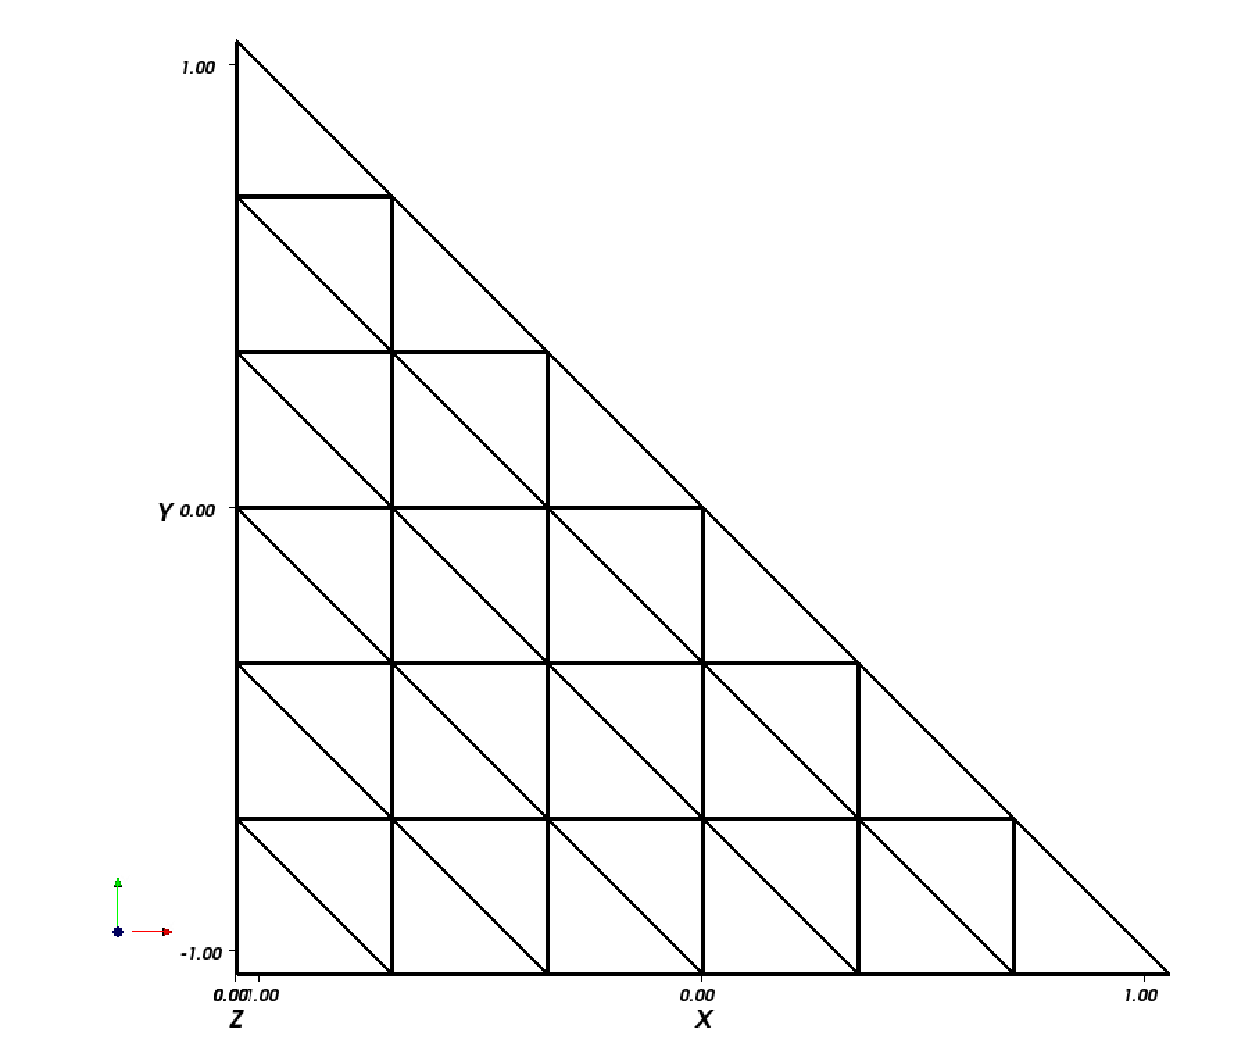
\includegraphics[width=0.7\textwidth]{../figures/triangle-equirepartis}\\
      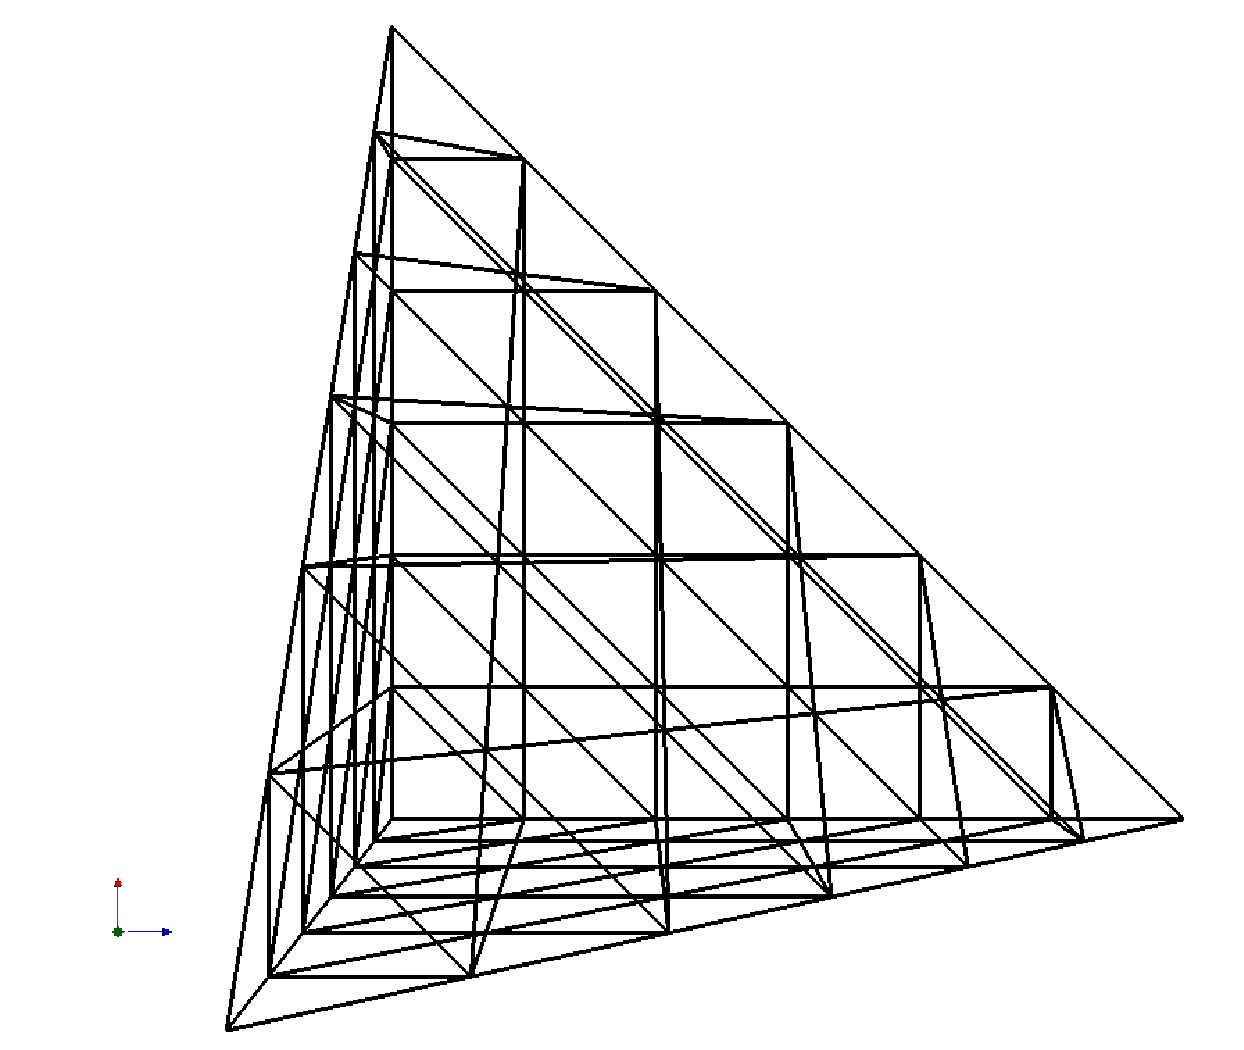
\includegraphics[width=0.7\textwidth]{../figures/tetra-equirepartis}
      \caption{\scriptsize Equi-distributed points in 2D/3D}
    \end{figure}
  \end{column}
  \begin{column}[c]{.6\textwidth}
    \begin{block}{Point Set $\{x_i\}_{i=1,N_p} \in K \subset \mathbb{R}^d$}
    \begin{itemize}
    \item Equi-distributed points
    \item Quadrature points, combination of
      \begin{itemize}
      \item Legendre
      \item Lobatto
      \item Radau
      \end{itemize}
    \item Interpolation points
      \begin{itemize}
      \item Fekete
      \item WarpBlend (explicit)
      \end{itemize}
    \item Algebraic representation: column oriented matrix ($d \times N_p$)
    \end{itemize}
    \hfill (Karniadakis \& Sherwin, Heasthaven, Warburton, Roth)
  \end{block}
  \end{column}
\end{columns}
\end{frame}
\begin{frame}{Construction}
  It is \alert{crucial} that all point sets are constructed with
  respect to the subentities of the reference domain for the DOF table
  construction ($C^0$ expansion or integration of faces)

  So if a point set of $N$ points in $\setR{d}$ is represented by a $d
  \times N $ matrix then
  \begin{itemize}
  \item first the points associated with vertices (wrt vertex ordering)
  \item then the points associated with the edges (wrt to edge ordering)
  \item  then the points associated with the faces (wrt to face ordering)
  \item  then the points associated with the volume
  \end{itemize}
\end{frame}

\subsection{Polynomial set}
\begin{frame}[label=pset]{Polynomials}

  Express the polynomials of $\Pk$ in the Dubiner basis $\{\phi_i\}_{i=1,\mathrm{dim} \Pk}$
    $$p=\sum_i (p, \phi_i)_K \phi_i,\quad p \in \Pk$$
    \begin{itemize}
    \item \alert{$L_2$ orthonormality}:
      \begin{itemize}
      \item exact integration,...
      \item Introduce $\mathcal{I} : \Pk \rightarrow \mathbb{R}^{\mathrm{dim} \Pk}$ such that
        for $p \in \Pk, i =1,\mathrm{dim} \Pk$
        $$(\mathcal{I}(p))_i = (p,\phi_i)_K = p_i$$
        $p \in \Pk$ is represented by $\mathcal{I}(p) = \mathbf{p} \in \mathbb{R}^{\mathrm{dim} \Pk}$ a row vector ($1 \times \mathrm{dim} \Pk$)
      \end{itemize}
%     \item \alert{Hierarchical Basis}
%       \begin{itemize}
%       \item Trivial to extract a basis of $\mathbb{P}_l(K) \subset \Pk, l \leq k$
%       \end{itemize}
    \end{itemize}
%  \note{Les propri�t�s math�matiques ($L_2$ orthonormal and  sont ici \alert{essentielles}}
\end{frame}

\begin{frame}{Polynomial Set}
  We now consider polynomial sets $P = \{p_i, i=1...N, p_i \in \Pk\}$.

  Again the polynomials are expressed in our $L_2$ orthonormal basis,
  ie
  \begin{equation}
    \label{eq:26}
    p_i = \sum_{k=1...\mathrm{dim}{\Pk}} p_{ik} \phi_k
  \end{equation}
  where $p_{ik}$ is the $k$-th component of the polynomial $p_i$.  We
  now wish to express our polynomial set $P$ in $\phi$, we just
  introduce the matrix $\mathbf{P}$

  \begin{equation}
    \label{eq:28}
    \mathbf{P} =(p_{ik})_{(i,k) \in [1...N]\times[1...\mathrm{dim}(\Pk)]}\}.
  \end{equation}

  The line $i$ of $\mathbf{P}$ holds the coefficients of the $i$-th polynomial.
\end{frame}

\begin{frame}[label=psetops]{Some Polynomial Set Operations}
  \begin{itemize}
  \item Addition, $\nabla \cdot$, $\nabla \times$ $L_2$ projection...
  \item Evaluation at a point set $X$: $V(P,X)$
    \begin{equation}
      \label{eq:35}
      V(P,X) = \mathbf{P}\ V( \phi, X )
    \end{equation}
    where $\phi$ is the basis in which $P$ is expressed.
  \item Derivate at a point set $X$: $V(\partial P,X)$
    \begin{equation}
      \label{eq:35}
      V(\partial P,X) = \mathbf{P}\ V( \partial \phi, X )
    \end{equation}
  \end{itemize}
\end{frame}

\begin{frame}[label=psetops]{Some Polynomial Set Operations}
  \begin{itemize}
  \item Integration $\int_{-1}^1 \phi_i(\xi)  d\xi$
    \begin{equation}
      \label{eq:34}
      \int_{-1}^1 \phi_i(\xi) d\xi = \sum_{q=1}^Q w_q \phi_i( \xi_q )
    \end{equation}
  \end{itemize}
\end{frame}

%   \begin{block}{Modal/Nodal Mapping }
%     \begin{itemize}
%     \item Given $X=\{x_j\}_{j=1,...,\mathrm{dim} \Pk}$ a point set in $K$
%     \item Given $V(\phi,X) = (\phi_i(x_j))$  Vandermonde matrix (modal/nodal coefficient mapping)
%     \item Given $\mathbf{p} \in \mathbb{R}^{\mathrm{dim} \Pk}$, such that $\mathbf{p} = \mathcal{I}(p)\, V(\phi,X)$
%     \end{itemize}

%   \end{block}
%   \begin{alertblock}{}
%     We look for $p$ that is to say we determine its  coefficients $\mathcal{I}(p)$ in the basis $(\phi_i)$
%   \end{alertblock}
% \end{frame}

% \begin{frame}{Differentatiation matrix}
%   \begin{example}{}
%     Given $D_l$ such that  $(D_l)_{i,j}= V(\frac{\partial \phi}{\partial x_l},Y)\ V^{-1}(\phi,Y)$, we have
%     \begin{equation}
%       \label{eq:13}
%       \mathcal{I}(\partial_l\ p) = \mathcal{I}( p )\ D_l
%     \end{equation}
%     The choice of $Y$ is crucial for good numerical stability.
%   \end{example}
%   \begin{alertblock}{Features}
%     Any order differentiation ($D_l^n$), Gradient, Divergence, Curl, $L_2$ projection
%   \end{alertblock}
% \end{frame}

\begin{frame}[containsverbatim]{C++ Polynomial and Polynomialset}
%\begin{lstlisting}[mathescape,basicstyle=\tiny\ttfamily]
\begin{lstlisting}[mathescape]
// Polynomial
template<typename Basis,
         typename PolyValueType >
class Polynomial {
 // basis from Poly (dimension N)
 // coefficients : matrix (nComponents x N)
};

// PolynomialSet
template<typename Basis,
         typename PolyValueType >
class PolynomialSet {...};

// OrthonormalPolynomialSet
template<uint16_type $d$,
  typename PolyValueType,
  typename T = double,
  template<uint16_type,uint16_type,
           uint16_type> class Convex>
class OrthonormalPolynomialSet {...};
\end{lstlisting}
\end{frame}

\begin{frame}[containsverbatim]{C++ Polynomial and Polynomialset}
\begin{lstlisting}[mathescape,basicstyle=\tiny\ttfamily]
// Scalar polynomial set
OrthonormalPolynomialSet<2,Scalar,Simplex> ScalarDubiner;
// Vectorial polynomial set
OrthonormalPolynomialSet<2,Vectorial,Simplex> VectorialDubiner;

// Scalar polynomial set
OrthonormalPolynomialSet<2,Scalar,SimplexProduct> ScalarLegendre;
// Vectorial polynomial set
OrthonormalPolynomialSet<2,Vectorial,SimplexProduct> VectorialLegendre;
\end{lstlisting}
\end{frame}

\begin{frame}[containsverbatim]{Polynomials Operations}

\begin{lstlisting}[mathescape,basicstyle=\tiny\ttfamily]
// Divergence $\nabla \cdot$
template<typename Basis>
PolynomialSet<Basis, Scalar>
div( PolynomialSet<Basis, Vectorial> const& p )
{
  const int nComponents =
   PolynomialSet<Basis, Vectorial>::nComponents;
  typedef typename Basis::value_type value_type;
  matrix<value_type> __div;
  for ( int i = 0; i <nComponents; ++i )  {
    __div += prod( p[i].coeff(),
                   p.basis().d(i) );
  }
   return PolynomialSet<Basis, Scalar>( Basis(), __div );
} // div
// $L_2$ Projection sur $\mathbb{P}$ = Pset
template<typename Pset, typename PExpr, typename IM>
Polynomial<Pset, Scalar>
project( Pset const& pset, PExpr const& expr, IM const& im )
{
  typedef typename PExpr::value_type value_type;
  // evaluate expr at quad nodes
  vector<value_type> exprq( expr( im.points() ) );
  // evaluate pset at quad nodes
  matrix<value_type> psetq( pset.evaluate( im.points() ) );
  return Polynomial<Pset, Scalar>(pset, prod( psetq, element_prod( exprq,
                                                                   im.weights() ) ) );
} // project
\end{lstlisting}
\end{frame}

\begin{frame}[containsverbatim]{Polynomial Operation II}
   \begin{columns}[t]
     \begin{column}{.5\textwidth}
  \begin{lstlisting}[mathescape,basicstyle=\tiny\ttfamily]
  template<typename P, typename PS,
   template<class, class> class Basis1,
   template<class, class> class Basis2 >
  PolynomialSet<P, PS>
  unite( Basis1<P, PS> const& pset1,
         Basis2<P, PS> const& pset2 )
  {
   // merge the two polynomial sets
   matrix<> M( pset1.coeff().size1()+
               pset2.coeff().size1(),
               pset1.coeff().size2() );
   project( M,
     range( 0, pset1.coeff().size1() ),
     range( 0,pset1.coeff().size2() ) ) =
                              pset1.coeff();
   project( M,
     range( pset1.coeff().size1(),
            pset1.coeff().size1()+
            pset2.coeff().size1() ),
     range( 0,pset1.coeff().size2() ) ) =
                              pset2.coeff();
   // SVD
   SVD<matrix<> > svd( M );
   // extract the submatrix of V
   matrix<> m (subrange( svd.V(),
                         0, svd.S().size(),
                         0, M.size2() ) );
   return PolynomialSet<>( P(), m ); }
  \end{lstlisting}
     \end{column}
     \begin{column}{.5\textwidth}
       \begin{block}{Base orthonormale de $\Hat{P} \subset P$}
         \begin{enumerate}
         \item Construire la base orthonormal de polyn�mes $\mathbb{P}$ r�sultant
           de l'union de $\mathbb{P}^a$ et $\mathbb{P}^b$ (i.e. $\mathbb{P}^a \oplus \mathbb{P}^b$)
         \item Faire une d�composition en valeur singuli�re $M = U S V^T$
         \item Extraire les lignes de $V$ associ�es aux valeurs singuli�res
           non-nulles
         \item Ces lignes forment les coefficients des polyn�mes qui
           engendrent l'espace polynomial r�sultant de $\oplus$
         \end{enumerate}
       \end{block}
     \end{column}
   \end{columns}
\end{frame}


\subsection[Functionals]{Functionals and Functional Sets $\Sigma$}

\begin{frame}{Linear Functionals}
  Consider now a linear functional $\sigma : \Pk \longrightarrow \mathbb{R}$
  Given $p \in \Pk$  and $(\phi_j)$ is a basis of $\Pk$, we have
  \begin{equation}
    \label{eq:20}
    \sigma(p) = \sum_{i=1}^{\mathrm{dim}(\Pk)} p_j \sigma(\phi_j)
  \end{equation}
  Introduce $\mathcal{J} : \mathcal{L}( \Pk, \mathbb{R}) \rightarrow \mathbb{R}^{\mathrm{dim}(\Pk)}$ and
  \begin{equation}
    \label{eq:21}
    (\mathcal{J}(\sigma))_j = (\sigma(\phi_j))
  \end{equation}
  In algebraic form, ($\mathcal{J}(\sigma)$ is a row vector), we have
  \begin{equation}
    \label{eq:22}
    \sigma( p ) = \langle \sigma, p \rangle = \underbrace{\mathcal{J}(\sigma)}_{1 \times \mathrm{dim} \Pk}\ \underbrace{\mathbf{p}^T}_{\mathrm{dim}\Pk \times 1 }\quad \text{(inner product)}
  \end{equation}
\end{frame}

\begin{frame}{Example: Functional evaluation at a point}
  Consider $\hat{x}_i \in \hat{K}$ and $\sigma_{\hat{x_i}}: p
  \rightarrow p(\hat{x_i})$.  $\sigma_{\hat{x_i}}$ is represented by
  the vector whose components are the evaluation of the basis
  functions $\phi_j$ at the point $\hat{x}_i$
  \begin{equation}
    \label{eq:23}
    (\mathcal{J}(\sigma))_j = ( \phi_j(\hat{x}_i) )
  \end{equation}
  if $\mathcal{J}(\sigma)$ is stored as a row vector ($1 \times \mathrm{dim}(\Pk)$), then
  \begin{equation}
    \label{eq:24}
    \sigma_{\hat{x_i}}(p) = \mathcal{J}(\sigma)\  \mathbf{p}^T\ =\ p(\hat{x}_i)\ (\in \setR{})
  \end{equation}


\end{frame}
\begin{frame}{Functional set}
  Similarly, a functional set
  $\Sigma=\{\sigma_i\}_{i=1...N}$ is represented by a matrix
  \begin{equation}
    \label{eq:25}
    (\sigma_i(\phi_j))_{i,j} \in \mathbb{R}^{N\times\mathrm{dim}(\Pk)}
  \end{equation}

  If $P$ is a polynomial set and $\Sigma$ a functional set, we have the matrix-matrix product
  \begin{equation}
    \label{eq:27}
    \underbrace{\Sigma}_{\text{matrix}} \underbrace{P^T}_{\text{matrix}}
  \end{equation}
  which is the application of the functional set onto the polynomial set.
\end{frame}



\begin{frame}[label=fsetops]{Some Functionals}
  \begin{block}{Functional $\sigma : \mathbb{P}(K) \longrightarrow \mathbb{R}$}
    \begin{itemize}
    \item Given $x_i \in K$, \\
      \alert{$\sigma_{x_i}: p \in \mathbb{P}(K) \longrightarrow p(x_i)$}
    \item Given $x_i \in K$ et $j=0,1,2$ derivation , \\
      \alert{$\sigma_{x_i,\, j}: p \in \mathbb{P}(K) \longrightarrow \frac{\partial p}{\partial x_j}(x_i)$}
    \item Given $q \in \mathbb{P}(K)$, \\
      \alert{$\sigma_{q}: p \in \mathbb{P}(K) \longrightarrow \int_K\ p\ q$}
    \item Given $\Gamma \subset \partial \Omega,\ q \in \mathbb{P}(K)$\\
      \alert{$\sigma_{\Gamma,\, q}: p \in \mathbb{P}(K) \longrightarrow \int_\Gamma\ p\ q$}
    \item Given $q \in \mathbb{P}(K)$,
      \alert{$\sigma_{\mathrm{div},\, q}: p \in [\mathbb{P}(K)]^d \longrightarrow \int_K\ \mathrm{div}( p )\ q$}
    \item ...
    \end{itemize}
  \end{block}
\end{frame}

\begin{frame}{Example: Lagrange polynomial construction}
  We now wish to construct the Lagrange polynomials expressed in our
  primal bases.

  \noindent
  Consider the point set  (equiadistributed, Gauss Lobatto...)
  \begin{equation}
    \label{eq:29}
    \{x_i, i =0...N\},
  \end{equation}
  we wish to construct the associated Lagrange polynomial set
  \begin{equation}
    \label{eq:30}
    H=\{h_j, j=0...N, h_j \in \PN\}
  \end{equation}
  Note that the $h_i$ will verify
  \begin{equation}
    \label{eq:31}
    h_j(x_i) = \delta_{ij},\quad i=0...N,\ j=0...N
  \end{equation}
  Introduce now
  \begin{equation}
    \label{eq:32}
    \Sigma=\{\sigma_{x_i}, \sigma_{x_i}(p) = p(x_i)\ i=0...N\}
  \end{equation}
  The matrix $H$ of coefficients of the polynomial set $H$ expressed
  in the basis $\phi$ verifies (see \ref{eq:31}), ie
  \begin{equation}
    \label{eq:33}
    \Sigma\ H^T = I
  \end{equation}
  where $I$ is the identity matrix, $\Sigma$ the matrix associated to
  the functional set. $H^T$ is the solution of a linear system.

\end{frame}


%% fset
\begin{frame}[containsverbatim]{Functionals }
\begin{lstlisting}[mathescape]
// $\sigma$
template<typename Space>
class Functional
{
 typedef Space polynomialset_type;
 typedef Space::polynomial_type polynomial_type;
 Functional( matrix<> coeff ) : {}
 void setCoefficient( matrix<> c )
 { _M_coeff = c; }
 // $\sigma( p )$
 matrix<> operator()( polynomial_type  p )
 {
   return prod( p.coeff(), trans(_M_coeff) );
 }
}
\end{lstlisting}
\end{frame}
\begin{frame}[containsverbatim]{Functional Sets}
\begin{lstlisting}[mathescape]
// $\Sigma$
template<typename Space>
class FunctionalSet
{
 typedef Space polynomialset_type;
 typedef Space::polynomial_type polynomial_type;
 FunctionalSet( vector<Functional<Space> funcs )
  {...}
 void setFunctionalSet(
                vector<Functional<Space> funcs )
 {...}
 // $\Sigma( p )$
 matrix<> operator()( polynomialset_type  p )
 {
   return prod( p.coeff(), trans(_M_coeff) );
 }
}
\end{lstlisting}
\end{frame}

%% fsetops
\begin{frame}[containsverbatim]{Some Functionnals}
\begin{lstlisting}[mathescape]
// Functional $\sigma_{x_i}$
template<typename Space>
class PointEvaluation
 : public Functional<Space>
{ ...
  PointEvaluation( Space const& b,
                   Point const& pt )
  :
  super( b, trans( b.basis()( pt )))
  {}
};


// Functional $\sigma_{x_i,\, j}$
template<typename Space>
class PointDerivative
 : public Functional<Space>
{ ...
  PointDerivative( Space const& b, int j,
                   Point const& pt )
  :
  super( b, b.basis().derivate(j).evaluate( pt ))
  {}
};
\end{lstlisting}
\end{frame}
\begin{frame}[containsverbatim]{Some Functionnals}
\begin{lstlisting}[mathescape]
// Functional $\sigma_{q}$
template<typename Space, typename Basis>
class IntegralMoment
 : public Functional<Space>
{
 IntegralMoment( Space const& p, Basis const& q )
 :
 super( p )
 {
   this->setCoefficient(
     prod( q.coeff(), trans( p.basis().coeff() ) ) );
 }
};
\end{lstlisting}
\end{frame}

\subsection{Applications}
\label{sec:applications}

\begin{frame}[label=apps]{FE construction}
  \begin{block}{}
    \begin{itemize}
    \item Dubiner, Legendre, and associated boundary adapted versions(cG)
    \item Lagrange (cG, dG, EF, ES)
    \item $\mathbb{P}_{1,2}$-Bubble
    \item Raviart-Thomas (2D, 3D)
    \item Nedelec
    \item Divergence Free
    \item Crouzeix-Raviart
    \item Hermite ($C^1$ element)
    \item Morley
    \item ...
    \end{itemize}
  \end{block}

  \begin{alertblock}{Key Ingredient}
    Hierarchical $L_2$ orthonormal  basis
  \end{alertblock}
\end{frame}


\begin{frame}[label=lag]{$(K,\ \mathbb{P}_k,\ \{\sigma_{x_i}\})$, $(K,\ [\mathbb{P}_k]^d,\ \{\sigma_{x_i}\})$}
  \begin{block}{Lagrange Finite Element}
          \begin{enumerate}
          \item Define $\Pk$
          \item Define $\Sigma=\{\sigma_{x_i}: \Pk \rightarrow \mathbb{R},\ x_i \in K\}$
          \item Order DOFs (continuous/discontinuous)
          \item Given $V$ associated with $\Sigma(\mathbb{P}_k)$,
            solve $V M = I$, $M^T$ contains the coefficients of the
            Lagrange polynomials in the basis of $\Pk$
          \end{enumerate}
      \end{block}
\end{frame}

\begin{frame}[fragile=singleslide]{$(K,\ \mathbb{P}_k,\ \{\sigma_{x_i}\})$, $(K,\ [\mathbb{P}_k]^d,\ \{\sigma_{x_i}\})$}
\begin{lstlisting}[mathescape,basicstyle=\tiny\ttfamily]
template<typename Primal,
         typename ContinuityType, // cG, dG
         class PointSetType>// $\{x_i\}$
class LagrangeDual
 : public DualBasis<Basis>
{
 LagrangeDual( primal_space_type const& primal )
 {
  PointSetType pts; // $\{x_i\}$
  if ( is_continuous )
   { ... } //reorder pts wrt entities

  setFunctionalSet( $\sigma_{\{x_i\}}$( primal, pts ) );
} };
template<uint16_type $d$,
         uint16_type $k$,
         class PolySetType,
         typename ContinuityType = Continuous,
         typename T = double,
         class Convex = Simplex,
         class Pts = PointSetEquiSpaced >
class Lagrange
 : public FiniteElement<
     OrthonormalPolynomialSet<$d$, $k$,
                  PolySetType, T, Convex>,
     LagrangeDual,
     ContinuityType,
     Pts >
{ Lagrange() : FiniteElement<>( dual(primal) ){} };
\end{lstlisting}
\end{frame}

\begin{frame}{$(K,\ \mathbb{P}_k,\ \{\sigma_{x_i}\})$, $(K,\ [\mathbb{P}_k]^d,\ \{\sigma_{x_i}\})$}
  \begin{figure}[H]
    \centering
    \subfigure{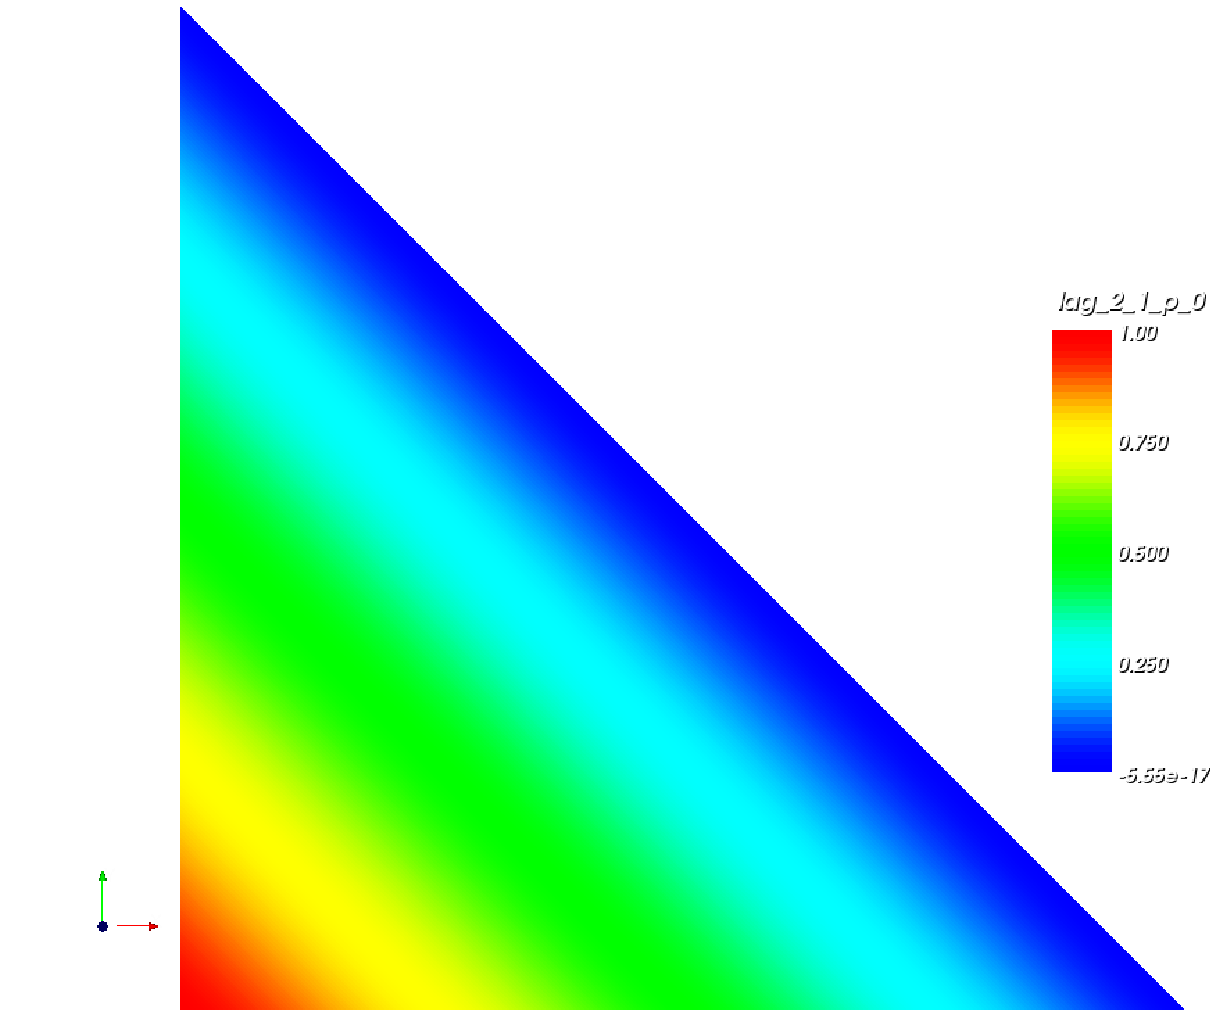
\includegraphics[width=.3\textwidth]{../figures/lag_2_1_p_0.pdf}}
    \subfigure{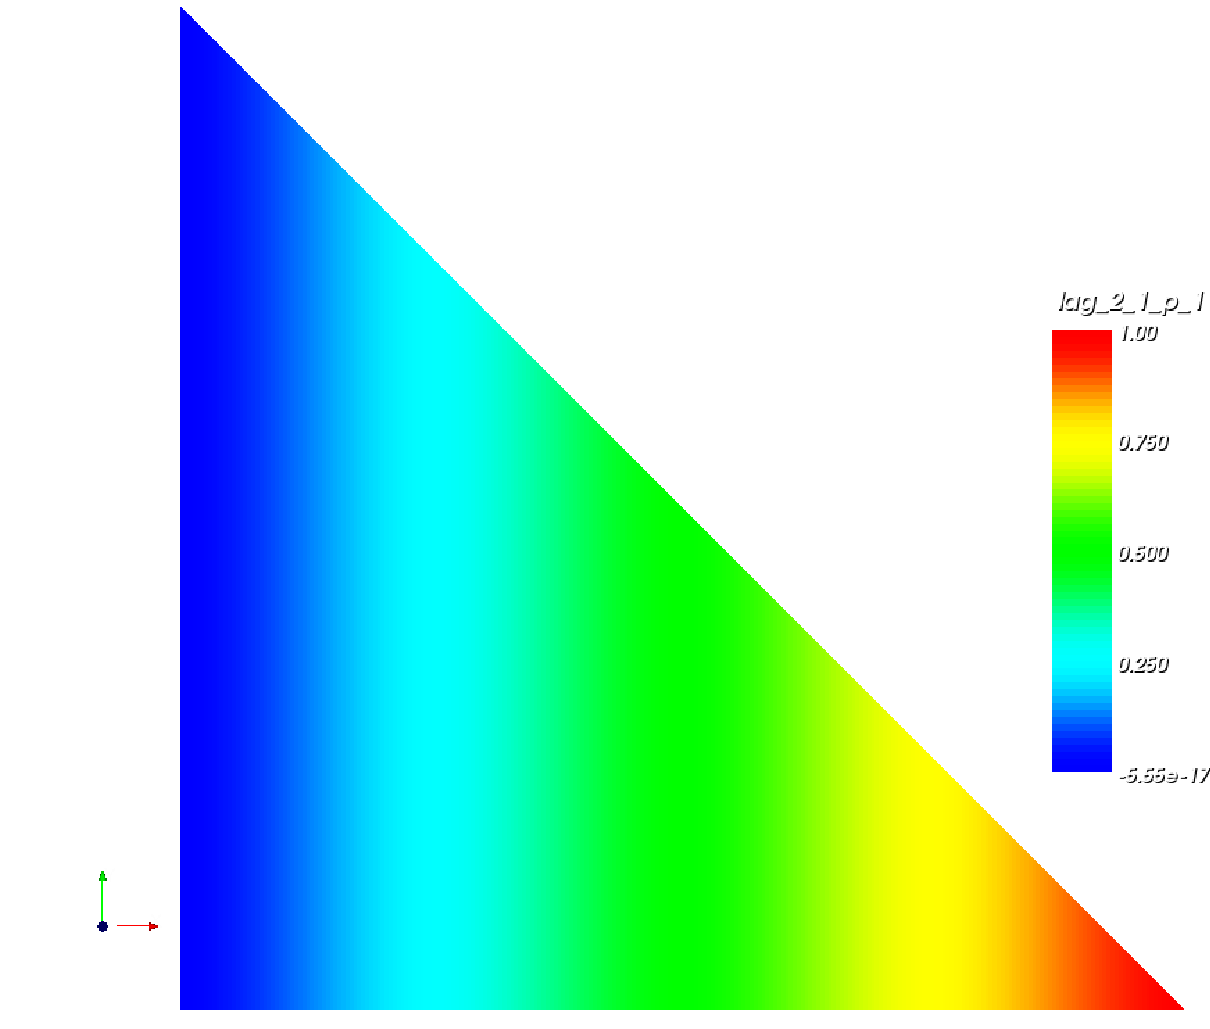
\includegraphics[width=.3\textwidth]{../figures/lag_2_1_p_1.pdf}}
    \subfigure{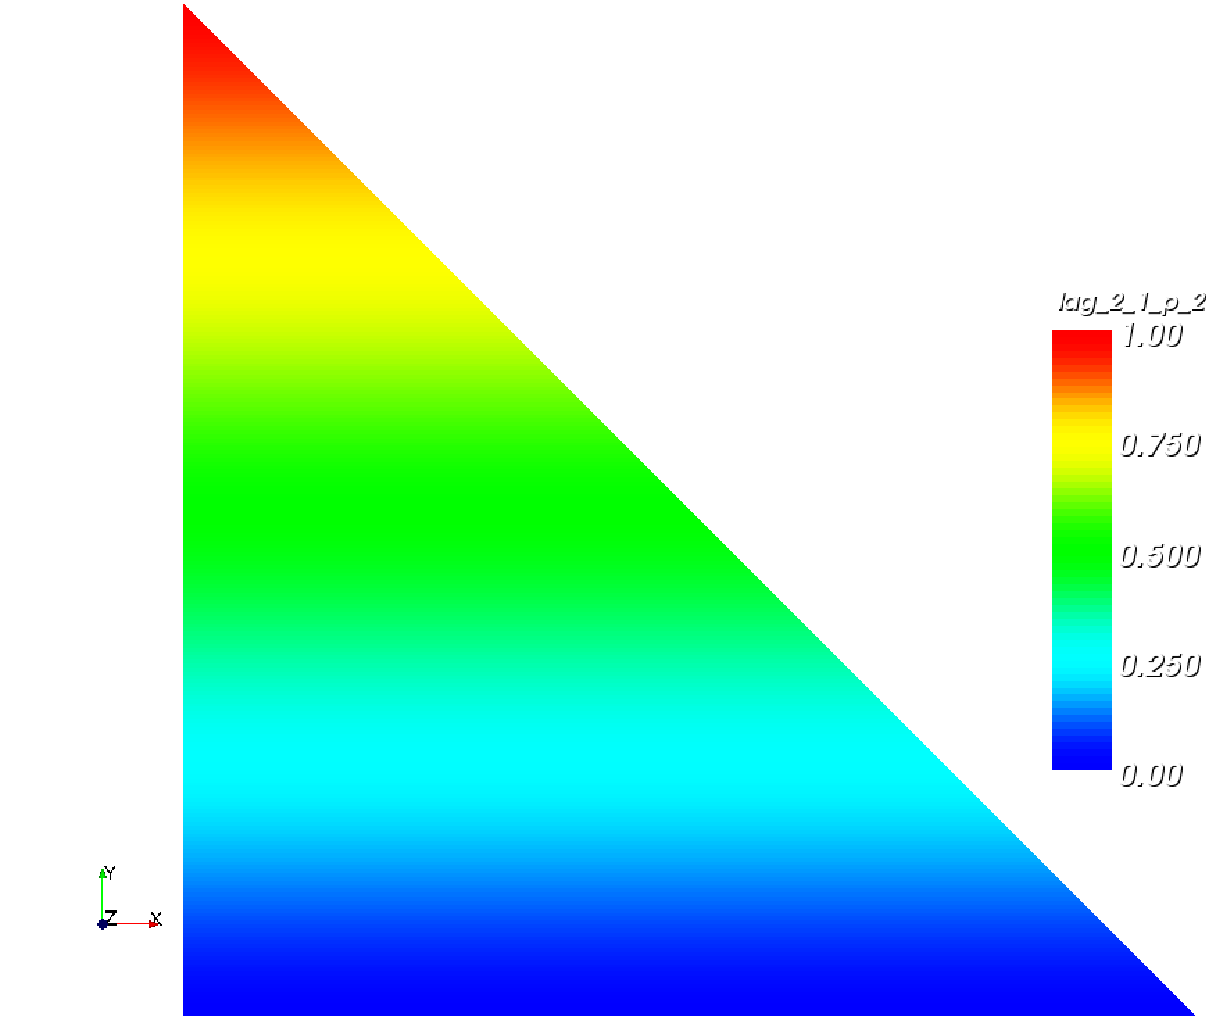
\includegraphics[width=.3\textwidth]{../figures/lag_2_1_p_2.pdf}}\\
    \subfigure{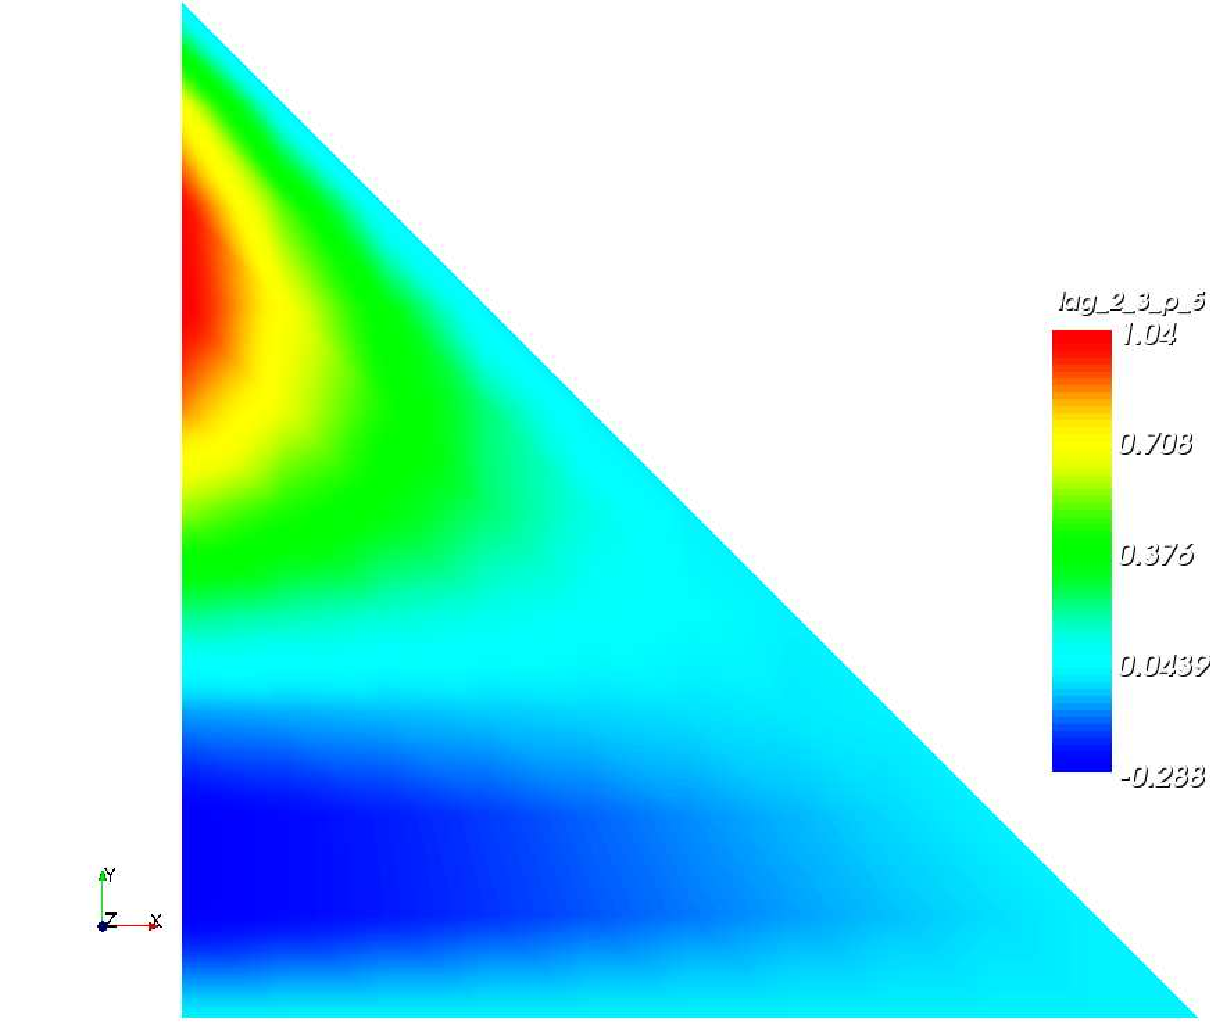
\includegraphics[width=.3\textwidth]{../figures/lag_2_3_p_5.pdf}}
    \subfigure{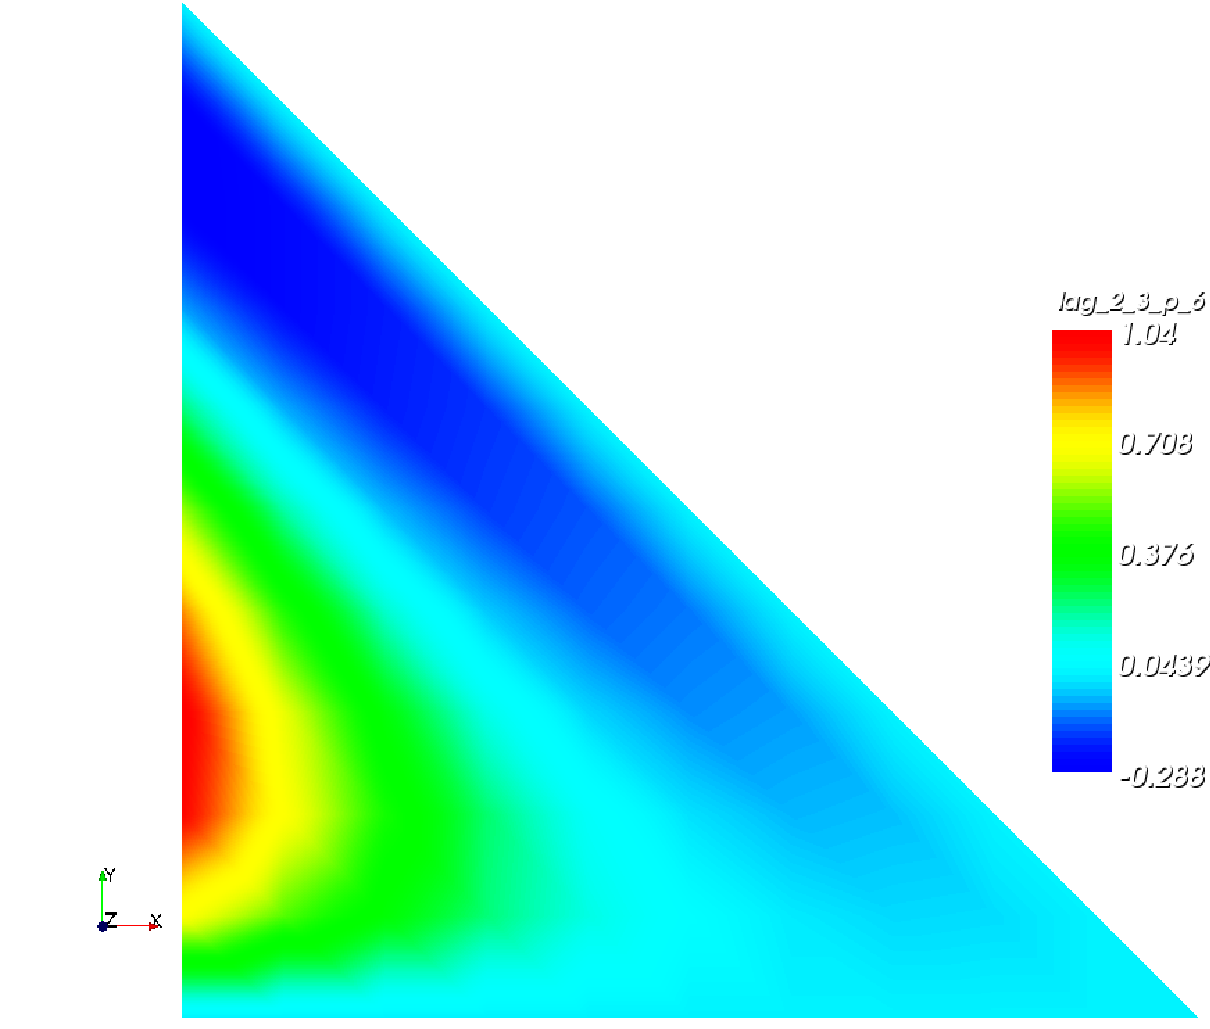
\includegraphics[width=.3\textwidth]{../figures/lag_2_3_p_6.pdf}}
    \subfigure{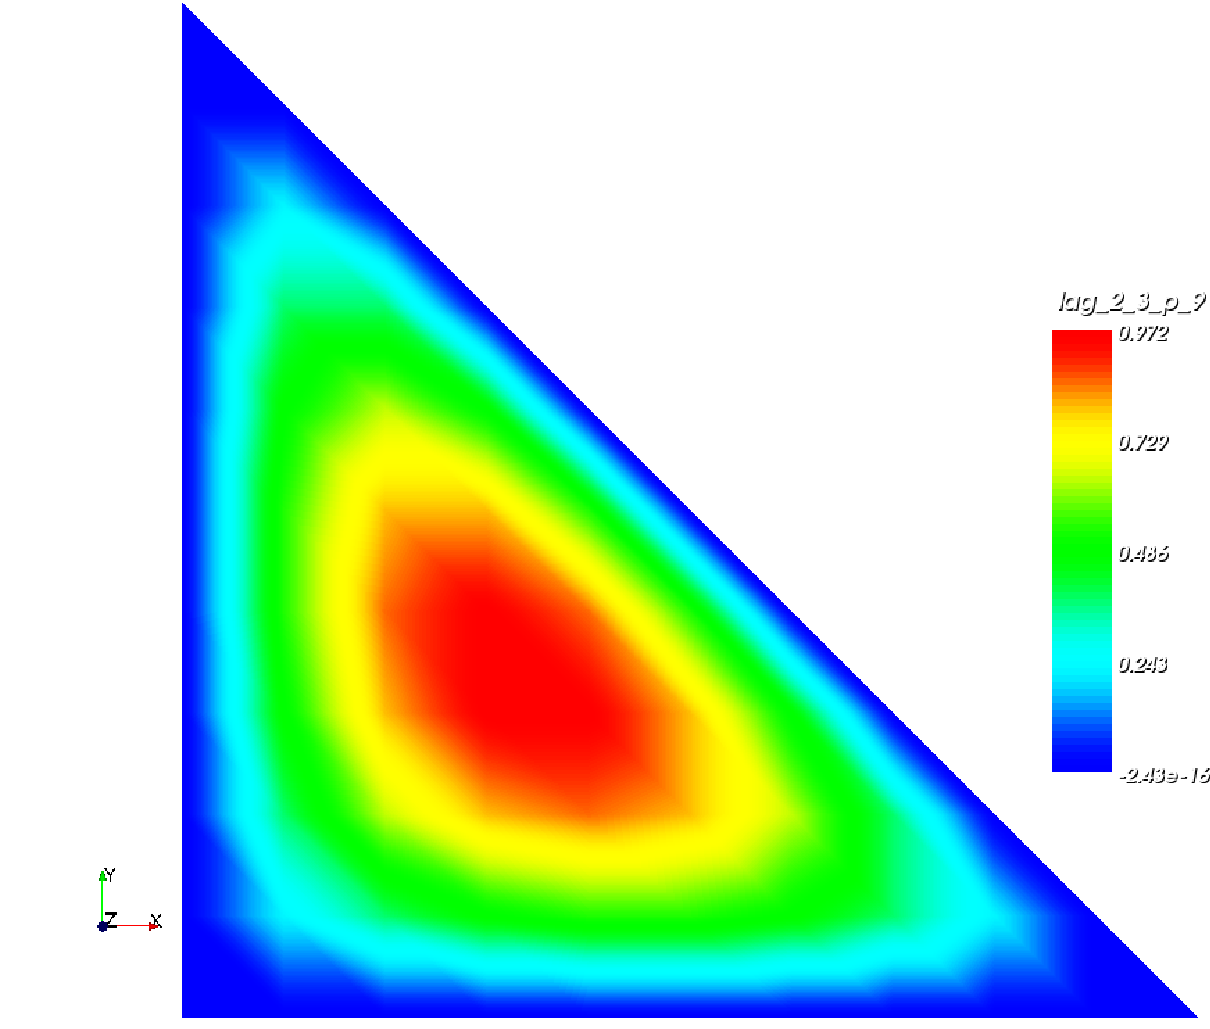
\includegraphics[width=.3\textwidth]{../figures/lag_2_3_p_9.pdf}}
    \caption{Scalar Lagrange element of order 1 (top). Some Lagrange polynomials of degree 3 (bottom)}
  \end{figure}
\end{frame}


\subsection{Multidomain extension}
\begin{frame}{what do we know?}
  \begin{itemize}
  \item We know how to write a variational formulation
  \item We know how to rewrite the integrals on each element region, as integrals on a reference element
  \item We know how to construct polynomial sets and do some
    operations (evaluation, integration,...) over the reference
    element
  \end{itemize}
\end{frame}

\begin{frame}{Problem: Laplacian equation}
  Consider now
  \begin{equation}
    \label{eq:36}
    \mathbb{L}(u) \equiv \frac{\partial^2 u}{\partial x^2} + f = 0, \quad f=-e^{-x},\ 0 \leq x \leq l
  \end{equation}
  and
  \begin{equation}
    \label{eq:39}
    \frac{\partial u}{\partial n}(0) = 1, \quad \frac{\partial u}{\partial n}(l) + u(l) = 0
  \end{equation}
  The exact solution is $g=e^{-x}$.


  If $u(x)$ and $v(x)$ are sufficiently smooth and we do integration by parts (Gauss theorem) and get
  \begin{equation}
\label{eq:37}
\int_0^l\ \frac{\partial u}{\partial x}\ \frac{\partial v}{\partial x}+  \int_0^l v f dx - \Big[ v\frac{\partial u}{\partial x}\Big]_0^l  = 0
  \end{equation}
  Denote then
  \begin{equation}
    \label{eq:38}
    \begin{array}[c]{rl}
      a(v, u) &= \int_0^1 \frac{\partial u}{\partial x}\ \frac{\partial v}{\partial x} + v(l)u(l)\\
      b(v) &= \int_0^l vf + v(0)
    \end{array}
  \end{equation}
  We look for $u \in \mathcal{X} \equiv \mathcal{V}$ such that
  \begin{equation}
    \label{eq:22}
    a(v,u) = b(v), \quad \forall v \in \mathcal{V}
  \end{equation}
\end{frame}
\begin{frame}{Discretisation}
  Consider a 1D mesh where the domain $\Om{}=[0,l]$ consists of
  $\nel$ elements and each element is of equal length
  $l/\nel$, ie $\Om{} = \cup_{e=1}^\nel\ \Om{e}$.

  Denote $\mathcal{V}^\delta = \{ p \in C^0(\Om{}), p_{|\Om{e}} \in \PN, e=1,..., \nel \}$.

  The problem now reads: find $u^\delta \in \mathcal{V}^\delta$ such that
  \begin{equation}
    \label{eq:27}
    a(v^\delta, u^\delta) = f(v^\delta)\ \forall\ v^\delta \in \mathcal{V}^\delta
  \end{equation}


\end{frame}

\begin{frame}{Algebraic form}
  We write now (\ref{eq:27}) taking $v^\delta = \Phi_i,
  i=1...\mathrm{dim}{\mathcal{V}^\delta}$ and express $u^\delta$ in
  the $\Phi$ basis, ie $u^\delta = \sum_{i=1}^\ndof u_i \Phi_i$ ($\ndof = \mathrm{dim} \mathcal{V}^\delta$)
  We thus get to solve the system
  \begin{equation}
    \label{eq:40}
    A u = b
  \end{equation}
  where
  \begin{itemize}
  \item $A_{ij} = \int_{0}^l \frac{\partial \Phi_j}{\partial x}\ \frac{\partial \Phi_i}{\partial x} dx + \Phi_i(l)\Phi_j(l), \quad i,j=1...\mathrm{dim} \mathcal{V}^\delta$
    \item $u = (u_j)_{j=1...\mathrm{dim} \mathcal{V}^\delta}$
    \item $b_i = \int_0^l \Phi_i fdx + \Phi_i(0)$
  \end{itemize}
\end{frame}
\begin{frame}{Geometric transformation}
  We introduce the geometric transformation  $\chi^e: \Omst \mapsto
  \Om{e}, \xi \rightarrow \chi^e(\xi )=x^e \in \Om{e}$ . We consider a linear
  transformation (ie $\chi^e(\xi) = a \xi + b$):
  \begin{equation}
    \label{eq:41}
    x^e = \chi^e(\xi) = \frac{1-\xi}{2} x^e_{e-1} + \frac{1+\xi}{2} x^e_e, \quad \xi \in \Omega^{\text{st}}, e = 1,...,\nel
  \end{equation}

  And since the elements are all the same size we have
  \begin{itemize}
  \item $K^e = \frac{h}{2}$ where $h=x^e_e - x^e_{e-1}$
  \item $J^e = \frac{h}{2}$
  \item $B^e = (K^e)^{-T} = \frac{2}{h}$
  \end{itemize}
\end{frame}
\begin{frame}{reformulation in reference element}
  Using the  formulas (end of first lecture)
  \begin{itemize}
  \item $A_{ij} = \sum_{e, (i,j) \in \Om{e}}
 \int_{-1}^1 \frac{2}{h}\frac{\partial \phi_\jloc}{\partial \xi}\ \frac{2}{h}\frac{\partial \phi_\iloc}{\partial \xi} \frac{h}{2}d\xi+ \phi_\iloc(1)\phi_\jloc(1)_{|e=\nel}, \quad i=\text{map}[e][\iloc], j=\text{map}[e][\jloc]$
    \item $u = (u_j)_{j=1...\mathrm{dim} \mathcal{V}^\delta}$
    \item $b_i = \sum_{e, (i) \in \Om{e}} \int_{-1}^1 \phi_\iloc(\xi) f(\chi^e(\xi)) \frac{h}{2}d\xi + \phi_\iloc(-1)_{|e=0}, \quad i=\text{map}[e][\iloc]$
  \end{itemize}

\end{frame}

\begin{frame}[containsverbatim]{element loop}
\begin{lstlisting}[mathescape]
for( int e = 0; e < nel; ++e )
{
  // compute $J^e$, $K^e$ and $B^e$

  // local assembly: compute integrals on $\Omst$

  // global assembly: assemble local matrix/vector into the global matrix
}
\end{lstlisting}
\end{frame}
\begin{frame}[containsverbatim]{Elementary matrix, vector}
  Denote $M^e$ the elementary matrix, it is constructed as follows
  \begin{lstlisting}[mathescape]
    for( int iloc = 0;iloc < $\nldof$; ++iloc )
     for( int jloc = 0;jloc < $\nldof$; ++jloc )
     {
      $M^e(\iloc,\jloc) = \int_{-1}^1 \frac{2}{h}\frac{\partial \phi_\jloc(\xi)}{\partial \xi}\ \frac{2}{h}\frac{\partial \phi_\iloc(\xi)}{\partial \xi} \frac{h}{2}d\xi $
      $M^e(\iloc,\jloc) = \sum_{q=1}^Q \frac{2}{h} w_q \frac{\partial \phi_\jloc(\xi_q)}{\partial \xi}\ \frac{2}{h}\frac{\partial \phi_\iloc(\xi_q)}{\partial \xi} \frac{h}{2}$;
      if ( e == $\nel-1$)
        $M^e(\iloc,\jloc) += \phi_\iloc(1)\phi_\jloc(1)$
     }
  \end{lstlisting}
  Likewise for $b^e$ the elementary vector
  \begin{lstlisting}[mathescape]
    for( int iloc = 0;iloc < $\nldof$; ++iloc )
     {
      $b^e(\iloc) = \int_{-1}^1 f(\chi^e(\xi)) \ \phi_\iloc(\xi) \frac{h}{2}d\xi = \sum_{q=1}^Q\ w_q f(x^e_q) \phi_\iloc(\xi_q) \frac{h}{2}$;
      if ( e == $0$ )
        $b^e(\iloc) += \phi_\iloc(-1)$
     }
  \end{lstlisting}
\end{frame}

\begin{frame}[containsverbatim]{DOF table}
  Consider now the case $N=1$ and $\nel=3$. We construct the associated dof table \lstinline!map!
  \begin{lstlisting}
    map[0] = {0, 1}
    map[1] = {1, 2}
    map[2] = {2, 3}
  \end{lstlisting}
  Consider now the case $N=2$ and $\nel=3$. We construct the associated dof table \lstinline!map!
  \begin{lstlisting}
    map[0] = {0, 1, 2}
    map[1] = {2, 3, 4}
    map[2] = {4, 5, 6}
  \end{lstlisting}
\end{frame}

\begin{frame}[containsverbatim]{Global Assembly}
  \begin{lstlisting}[mathescape]
  for( int iloc = 0;iloc < $\nldof$; ++iloc )
  {
    int i = map[e][$\iloc$];
     for( int jloc = 0;jloc < $\nldof$; ++jloc )
     {
       int j = map[e][$\jloc$];
       A( i, j ) += $M^e(\iloc, \jloc)$;
     }
     b( i ) += $b^e(\iloc)$;
  }
  \end{lstlisting}
\end{frame}

% \begin{frame}{Case $N=1$, $\nel=3$}
%   We get the matrix
%   \begin{equation}
%     \label{eq:42}A=
%     \begin{pmatrix}
%       \frac{4}{h} & \frac{4}{h} & & \\
%       \frac{4}{h} & \frac{4}{h} & \frac{4}{h} &\\
%       & \frac{4}{h} & \frac{4}{h} & \frac{4}{h} \\
%       & & \frac{4}{h} & \frac{4}{h}+1 \\
%     \end{pmatrix}
%   \end{equation}
%   and
%   \begin{equation}
%     \label{eq:43}
%     \begin{pmatrix}
%       1 + \ \sum_{q=1}^Q w_q (-e^{x^0_q}) \phi_0(\xi_q) \frac{h}{2}\\
%       \sum_{q=1}^Q w_q (-e^{x^0_q}) \phi_1(\xi_q) \frac{h}{2} + \sum_{q=1}^Q w_q (-e^{x^1_q}) \phi_0(\xi_q) \frac{h}{2}\\
%       \sum_{q=1}^Q w_q (-e^{x^1_q}) \phi_0(\xi_q) \frac{h}{2} + \sum_{q=1}^Q w_q (-e^{x^2_q}) \phi_0(\xi_q) \frac{h}{2}\\
%       \sum_{q=1}^Q w_q (-e^{x^2_q}) \phi_1(\xi_q) \frac{h}{2}\\
%     \end{pmatrix}
%   \end{equation}
% \end{frame}
\section{Life}
\subsection{Architecture}
\begin{frame}[plain]{Architecture}
  \mode<article>{\includegraphics[width=\textwidth]{../../../../../../figures/arch2}}
  \mode<beamer>{\includegraphics[height=.9\textheight]{../../../../../../figures/arch2}}
\end{frame}


\end{document}
\subsection{Newton}
\label{sec:newton}

\begin{frame}{}

\end{frame}

\section[Lagrange]{Lagrange basis}
\label{sec:lagrange-basis}

\subsection{Interpolation}
\label{sec:interpolation}


\begin{frame}{}

\end{frame}

\subsection{Runge Phenomenon}
\label{sec:runge-phenomenon}

\begin{frame}{}

\end{frame}

\subsection{Chebyshev polynomials}
\label{sec:chebysh-polyn}

\begin{frame}{}

\end{frame}

\subsection[Interval]{Interval Approximation}
\label{sec:interv-interp}

\begin{frame}{}

\end{frame}


\section{Multidimension approximation}
\label{sec:mult-interp}

\subsection{Basic geometry}
\label{sec:basic-geometry}

\begin{frame}{}

\end{frame}

\subsection{Coordinate systems}
\label{sec:coordinate-systems}

\begin{frame}{}

\end{frame}

\subsection{Primal basis}
\label{sec:primal-basis}

\begin{frame}{}

\end{frame}

\subsection{Polynomials and set of polynomials}
\label{sec:polyn-set-polyn}

\begin{frame}{}

\end{frame}

\subsection{Functionals and sets of functionals}
\label{sec:functionals}

\begin{frame}{}

\end{frame}

\subsection{Finite elements}
\label{sec:finite-elements}

\begin{frame}{}

\end{frame}

\subsection{Geometric Transformation}
\label{sec:geom-transf}

\begin{frame}{}

\end{frame}

\subsection{Curvilinear domain}
\label{sec:curvilinear-domain}

\begin{frame}{}

\end{frame}


\section{Other Representations}
\label{sec:other-repr}

\subsection{Fourier}
\label{sec:fourier-polynomials}

\begin{frame}{}

\end{frame}


\subsection{Wavelets}
\label{sec:wavelets}

\begin{frame}{}

\end{frame}

\section{MPI}
\label{sec:mpi}

\subsection{Send/Recv}
\label{sec:sendrecv}

\begin{frame}{}

\end{frame}

\section{Programming}
\label{sec:programming}

\subsection{MPI Send/Recv}
\label{sec:mpi-sendrecv}

\begin{frame}{}

\end{frame}

\subsection{C++}
\label{sec:c++}

\begin{frame}{}

\end{frame}

\subsection{Libraries}
\label{sec:libraries}

\begin{frame}{}

\end{frame}



\end{document}


%%% Local Variables:
%%% mode: latex
%%% TeX-master: "scicomp-approx-print"
%%% TeX-PDF-mode: t
%%% TeX-parse-self: t
%%% x-symbol-8bits: nil
%%% TeX-auto-regexp-list: TeX-auto-full-regexp-list
%%% ispell-local-dictionary: "american"
%%% End:

